\section{Interfacing the Ninebot Go-kart PRO's control system}
\label{sec:Interfacing the Ninebot Go-kart PROs control system}
The Ninebot Go-kart PRO is a widely available consumer-grade electric go-kart.
It is build in a modular way, extending a standard Ninebot S MAX balance board to a go-kart by adding a frame with a remote controller located inside the cart's steering column which connects to the balance board.
As the product was not intended to be modified by the end user and closed-source during the project's development phase, there was no official option to interface with its control system.
Reverse engineering was executed for investigating possible ways how the go-cart's brake signal could be manipulated.

\subsection{Architecture of the Go-Kart's Remote Controller}
In a first step, the remote controller was taken apart and analyzed.
It was found out that it acts as an encapsulated system with an independent power supply in form of batteries which are also located inside the steering column.
The system uses a nRF51822 System On Chip (SoC) from Nordic Semiconductor for processing the gas and brake pedals' signals and communicating with the balance board.
Both gas and brake pedal utilize a hall sensor to output an analog voltage proportional to the position of the pedal's lever, which is converted from analog to digital domain by using the SoC's internal Analog to Digital Converter (ADC).
\begin{figure}[!htbp]
\centering
\begin{subfigure}{0.24\textwidth}
  \centering
  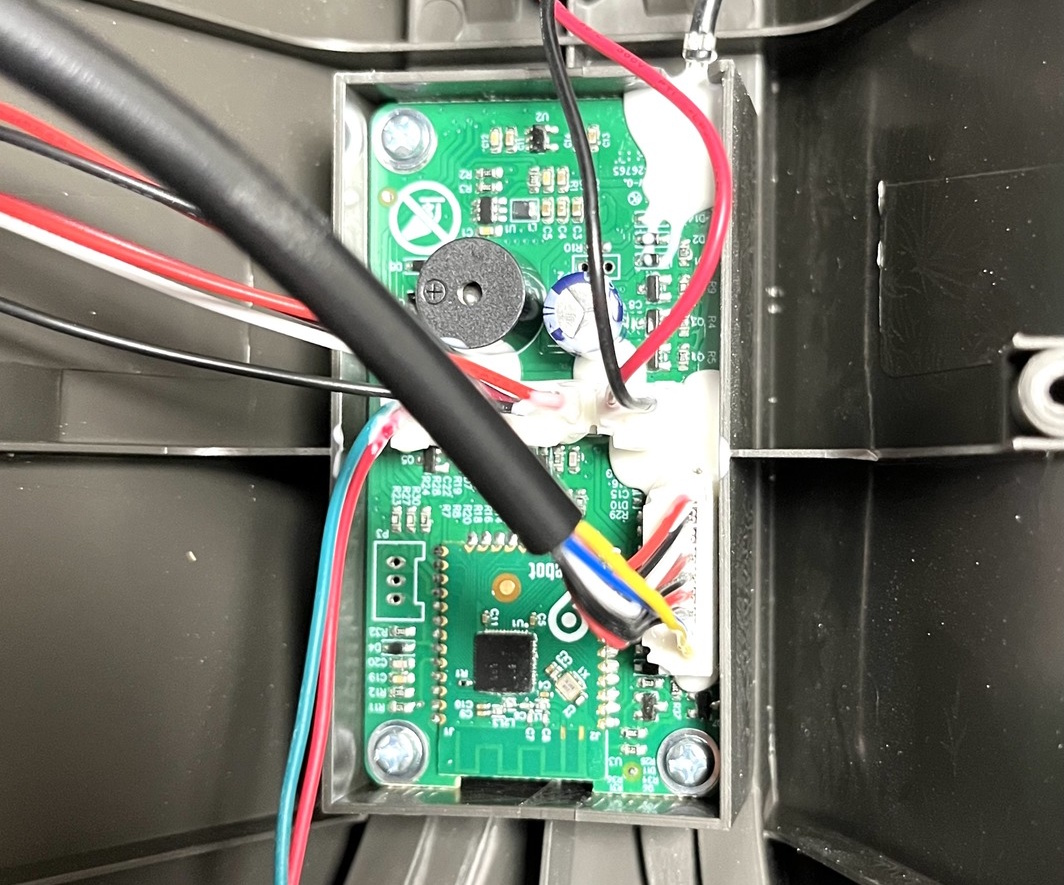
\includegraphics[width=\textwidth]{images/remote_controller_board2.jpg}
\end{subfigure}
\begin{subfigure}{0.24\textwidth}
  \centering
  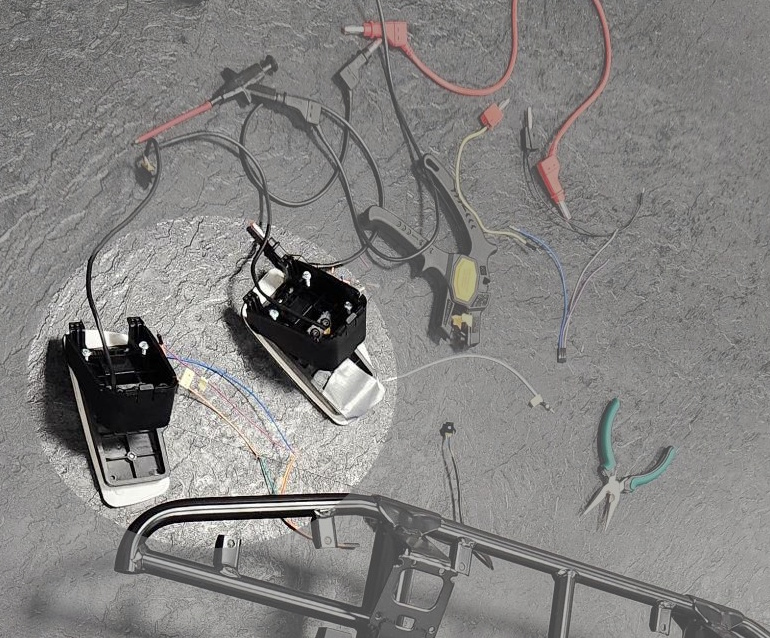
\includegraphics[width=\textwidth]{images/gas_and_brake_pedals.jpg}
\end{subfigure}
\caption{The remote controller's board inside the steering column and the dismantled brake-pedals.}
\label{fig:remote_controller_components}
\end{figure}
\FloatBarrier\noindent
These signals are passed from the remote controller to the balance board by using two separate communication channels: a wired connection through a cable inside the go-kart's frame and a wireless connection via Bluetooth is used \cite{ninebot_product_page}.
Multiple sources of documented successfully reverse engineered wireless communication interfaces of older Ninebot scooters stated that a proprietary protocol using a virtual UART at a speed of \SI{115200}{\baud}, without parity-bits and with $1$ stop-bit, was used for the wireless communication \cite{ninebot_protocol_github}\cite{ninebot_protocol_scooterhacking}.
\par
Tracing the pins which are used by the wired connection on the remote controller's Printed Circuit Board (PCB) and the labeling on the PCB's backside ("RXD" and "TXD") also suggested a UART connection.
These findings implied three possible ways of taking over the control of the brake pedal's signal:
\begin{enumerate}
    \item Reverse engineering and manipulating the communication of the wired UART connection.
    \item Manipulating the analog signal of the brake pedal.
    \item Reverse engineering and manipulating the wireless communication protocol of the Bluetooth virtual UART connection.
\end{enumerate}
As manipulating the brake signal via the wired UART connection posed to be the second simplest way while potentially offering more possibilities of getting control of the go-kart or obtaining information from it, compared to the approach of manipulating the analog signal, this way was investigated first.
\par
A Digital Storage Oscilloscope (DSO) with an integrated UART decoder was connected to the data lines to be examined.
According to the resources, a \SI{2}{\byte} long frame header with the sequence "$0x5A$ $0xA5$"
should have been present at the beginning of each packet\cite{ninebot_protocol_scooterhacking}.
All possible combinations of the UART decoder regarding speed, polarity, parity-bits, and stop-bits were tested but none showed the expected frame header.
Additionally, the presence of big voltage spikes with an amplitude of up to \SI{4}{\volt}, dependent on the motor's Revolutions Per Minute (RPM), was discovered.
\par
In a second test, it was investigated whether there was a dependency between the frames sent and the value of the gas and brake signal.
For this test, the rising edge of the brake pedal's analog signal output was used to trigger the DSO's capture event.
The pedal was slowly pressed, kept fully pressed for approximately \SI{175}{\milli\second} time and then was released again.
This procedure yielded the recording of a communication sequence over a longer period of time.
It was carefully checked for dependencies between the brake signal and the frames' contents and the periodicity of communication events, but there was no evidence of correlation.
\begin{figure}[!htbp]
\centering
  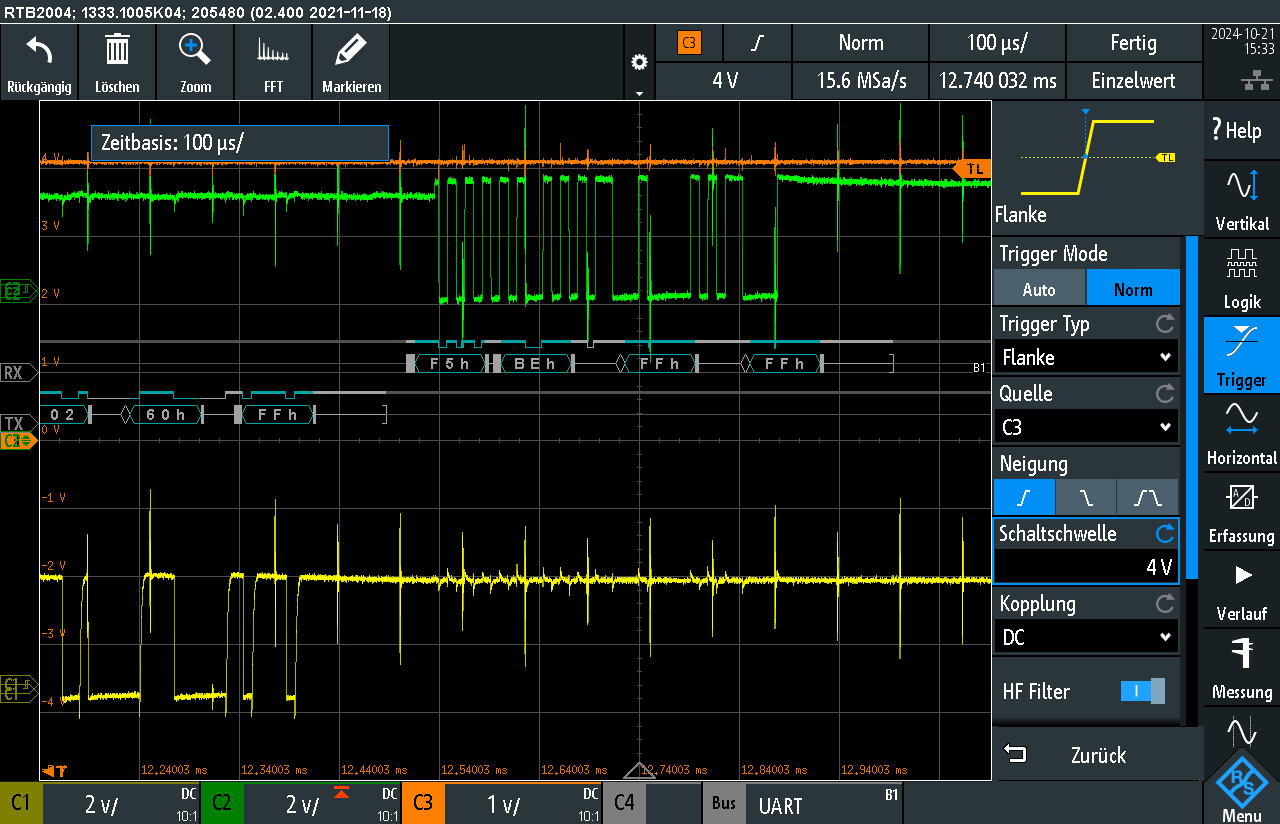
\includegraphics[width=0.48\textwidth]{images/uart_dso_1.png}
\caption{Plot of the communication between the remote controller and the balance board in idle. Voltage spikes of up to \SI{4}{\volt} can be observed.}
\label{fig:dso_uart_plot1}
\end{figure}
\FloatBarrier\noindent
\begin{figure}[!htbp]
\centering
  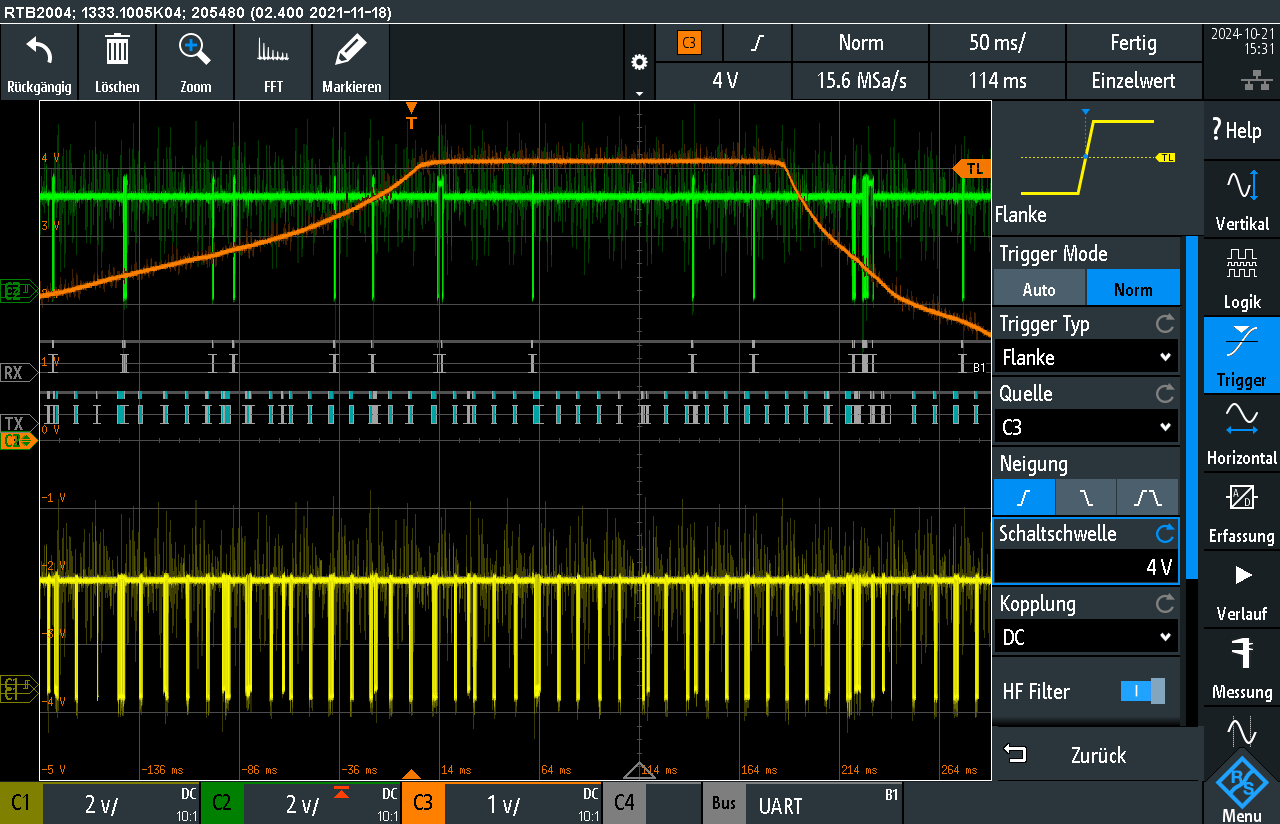
\includegraphics[width=0.48\textwidth]{images/uart_dso_2.png}
\caption{Plot of the communication between the remote controller and the balance board while using the brake pedal's analog signal as the trigger.}
\label{fig:dso_uart_plot2}
\end{figure}
\FloatBarrier\noindent
\par
Because no source explicitly stated that the wired connection was used for exchanging gas and brake signals, two last tests were executed.
In the first test, the go-kart was powered up with the wired connection between the remote controller and the balance board being detached beforehand.
The go-kart refused to enter its normal operating mode and stayed in a "safety-mode" until power was cycled with the wired connection re-attached.
In the second test, the go-kart was powered up normally and the wired connection was detached while it was already in its normal operating mode.
The go-kart continued to operate normally, fully relying on the wireless communication for the transmission of gas and brake signals.
The results of these tests led to the assumption that the wired connection is not used for the transmission of gas and brake signals or only as a fallback option if the wireless communication is disrupted during normal operation.
Since deliberately blocking the wireless connection was not possible and fully replacing the remote controller not an option, the manipulation of the brake signal was performed by overwriting the pedal's analog voltage.

\subsection{Interfacing the Brake Pedal}
The brake pedal outputs a voltage in the range of \SIrange{1.2}{4.2}{\volt} which is proportional to the position of the pedal's lever (see \ref{fig:dso_uart_plot2}, orange plot).
As the brake pedal's signal has priority over the gas pedal's signal (the go-kart stops if both pedals are pressed simultaneously), it is sufficient to overwrite its signal by the emergency braking system in case of an emergency braking event.
Overwriting can be done by adding the two signals together and feeding the result into the remote controller's input.
The signal needs to be clipped at the maximum input level of \SI{4.2}{\volt}, to protect the remote SoC's analog inputs from overvoltage.
A simplistic design incorporating three operational amplifiers was developed for implementing these stages:
\begin{figure}[!htbp]
\centering
  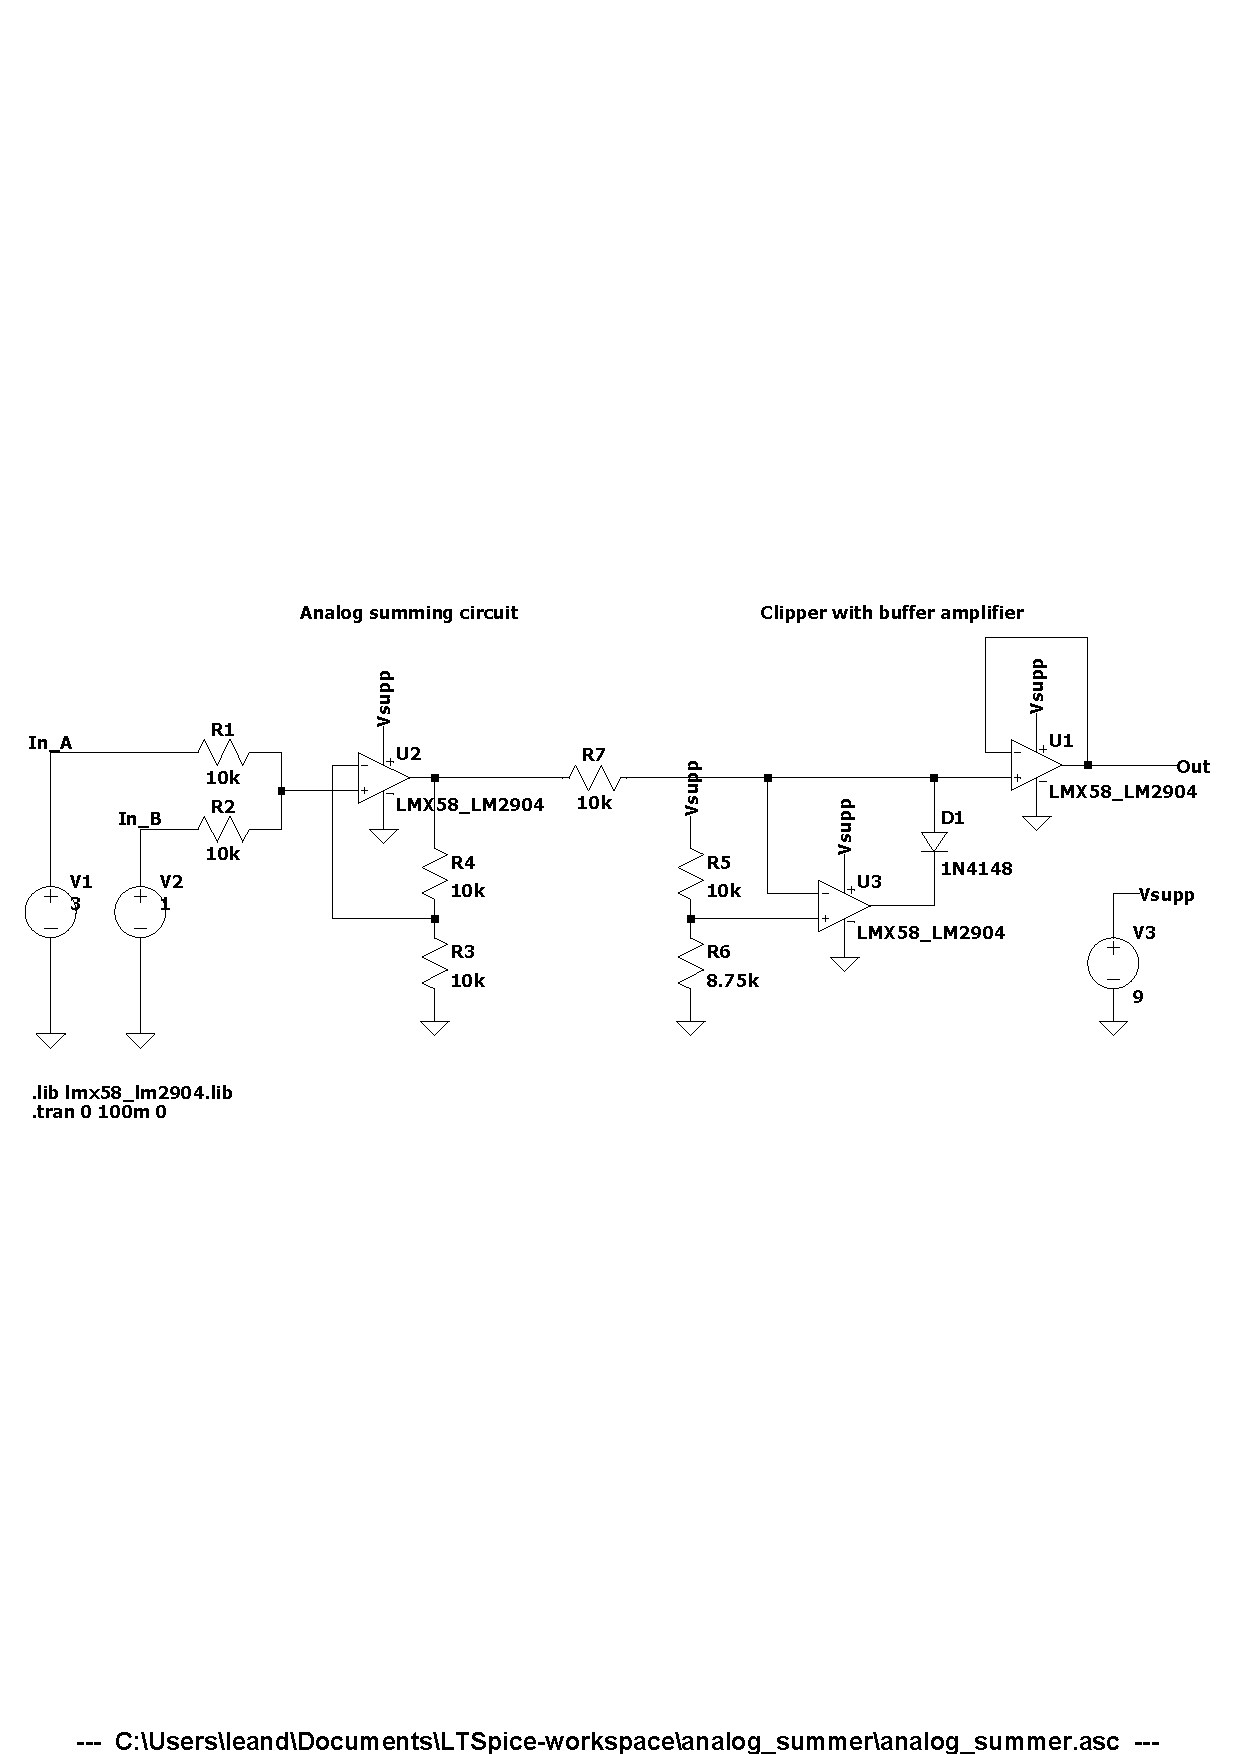
\includegraphics[trim=0cm 11cm 0cm 10cm, clip, width=0.48\textwidth]{images/analog_summer.pdf}
\caption{Analog summing circuit followed by a clipper and a buffer amplifier}
\label{fig:analog_summer}
\end{figure}
\FloatBarrier\noindent
A buffer amplifier (voltage follower) was added to lower the circuit's output impedance and to mitigate the influence of the connected load on the clipping voltage.
The insertion of this circuit between the brake pedal's output and the remote controller's input allows the emergency braking system to overwrite the brake signal to initiate a braking event while keeping the pedal's normal functionality.